\documentclass[twoside]{book}

% Packages required by doxygen
\usepackage{fixltx2e}
\usepackage{calc}
\usepackage{doxygen}
\usepackage[export]{adjustbox} % also loads graphicx
\usepackage{graphicx}
\usepackage[utf8]{inputenc}
\usepackage{makeidx}
\usepackage{multicol}
\usepackage{multirow}
\PassOptionsToPackage{warn}{textcomp}
\usepackage{textcomp}
\usepackage[nointegrals]{wasysym}
\usepackage[table]{xcolor}

% Font selection
\usepackage[T1]{fontenc}
\usepackage[scaled=.90]{helvet}
\usepackage{courier}
\usepackage{amssymb}
\usepackage{sectsty}
\renewcommand{\familydefault}{\sfdefault}
\allsectionsfont{%
  \fontseries{bc}\selectfont%
  \color{darkgray}%
}
\renewcommand{\DoxyLabelFont}{%
  \fontseries{bc}\selectfont%
  \color{darkgray}%
}
\newcommand{\+}{\discretionary{\mbox{\scriptsize$\hookleftarrow$}}{}{}}

% Page & text layout
\usepackage{geometry}
\geometry{%
  a4paper,%
  top=2.5cm,%
  bottom=2.5cm,%
  left=2.5cm,%
  right=2.5cm%
}
\tolerance=750
\hfuzz=15pt
\hbadness=750
\setlength{\emergencystretch}{15pt}
\setlength{\parindent}{0cm}
\setlength{\parskip}{3ex plus 2ex minus 2ex}
\makeatletter
\renewcommand{\paragraph}{%
  \@startsection{paragraph}{4}{0ex}{-1.0ex}{1.0ex}{%
    \normalfont\normalsize\bfseries\SS@parafont%
  }%
}
\renewcommand{\subparagraph}{%
  \@startsection{subparagraph}{5}{0ex}{-1.0ex}{1.0ex}{%
    \normalfont\normalsize\bfseries\SS@subparafont%
  }%
}
\makeatother

% Headers & footers
\usepackage{fancyhdr}
\pagestyle{fancyplain}
\fancyhead[LE]{\fancyplain{}{\bfseries\thepage}}
\fancyhead[CE]{\fancyplain{}{}}
\fancyhead[RE]{\fancyplain{}{\bfseries\leftmark}}
\fancyhead[LO]{\fancyplain{}{\bfseries\rightmark}}
\fancyhead[CO]{\fancyplain{}{}}
\fancyhead[RO]{\fancyplain{}{\bfseries\thepage}}
\fancyfoot[LE]{\fancyplain{}{}}
\fancyfoot[CE]{\fancyplain{}{}}
\fancyfoot[RE]{\fancyplain{}{\bfseries\scriptsize Generated by Doxygen }}
\fancyfoot[LO]{\fancyplain{}{\bfseries\scriptsize Generated by Doxygen }}
\fancyfoot[CO]{\fancyplain{}{}}
\fancyfoot[RO]{\fancyplain{}{}}
\renewcommand{\footrulewidth}{0.4pt}
\renewcommand{\chaptermark}[1]{%
  \markboth{#1}{}%
}
\renewcommand{\sectionmark}[1]{%
  \markright{\thesection\ #1}%
}

% Indices & bibliography
\usepackage{natbib}
\usepackage[titles]{tocloft}
\setcounter{tocdepth}{3}
\setcounter{secnumdepth}{5}
\makeindex

% Hyperlinks (required, but should be loaded last)
\usepackage{ifpdf}
\ifpdf
  \usepackage[pdftex,pagebackref=true]{hyperref}
\else
  \usepackage[ps2pdf,pagebackref=true]{hyperref}
\fi
\hypersetup{%
  colorlinks=true,%
  linkcolor=blue,%
  citecolor=blue,%
  unicode%
}

% Custom commands
\newcommand{\clearemptydoublepage}{%
  \newpage{\pagestyle{empty}\cleardoublepage}%
}

\usepackage{caption}
\captionsetup{labelsep=space,justification=centering,font={bf},singlelinecheck=off,skip=4pt,position=top}

%===== C O N T E N T S =====

\begin{document}

% Titlepage & ToC
\hypersetup{pageanchor=false,
             bookmarksnumbered=true,
             pdfencoding=unicode
            }
\pagenumbering{roman}
\begin{titlepage}
\vspace*{7cm}
\begin{center}%
{\Large Wa-\/tor }\\
\vspace*{1cm}
{\large Generated by Doxygen 1.8.11}\\
\end{center}
\end{titlepage}
\clearemptydoublepage
\tableofcontents
\clearemptydoublepage
\pagenumbering{arabic}
\hypersetup{pageanchor=true}

%--- Begin generated contents ---
\chapter{Wat-\/tor Simulation}
\label{md_README}
\hypertarget{md_README}{}
This is a short program used to simulate the conditions and relationship between sharks and fishes in an ecosystem. It is being developed in C++, and Open\+Mp. 



\subsection*{Files }

Wa-\/tor.\+cpp

\begin{quote}
{\bfseries Note\+:} \end{quote}


\begin{quote}

\begin{DoxyItemize}
\item This is the main application source file. 
\end{DoxyItemize}\end{quote}


\hyperlink{_animal_8cpp}{Animal.\+cpp}

\begin{quote}
{\bfseries Note\+:} \end{quote}


\begin{quote}

\begin{DoxyItemize}
\item This is used to differentiate between a fish, shark, or water. 
\end{DoxyItemize}\end{quote}


\hyperlink{_animal_8h}{Animal.\+h}

\begin{quote}
{\bfseries Note\+:} \end{quote}


\begin{quote}

\begin{DoxyItemize}
\item Header file for \hyperlink{_animal_8cpp}{Animal.\+cpp} 
\end{DoxyItemize}\end{quote}


Makefile

\begin{quote}
{\bfseries Note\+:} \end{quote}


\begin{quote}

\begin{DoxyItemize}
\item Uses g++ to compile and debug C++ code 
\end{DoxyItemize}\end{quote}


\paragraph*{{\itshape } Code running in serial}

Graphs will be put here

\paragraph*{{\itshape } Code running in parrallel}

\begin{quote}
{\bfseries System Specs\+:} \end{quote}


\begin{quote}

\begin{DoxyItemize}
\item Ram \+: 3541
\item Processor \+: Intel(\+R) Core(\+T\+N) i7-\/4700\+HQ C\+PU @ 2.\+40\+G\+Hz
\item OS \+: Ubuntu 
\end{DoxyItemize}\end{quote}


(35 x 60) Size of World



(18 x 30) Size of World

 
\chapter{Namespace Index}
\section{Namespace List}
Here is a list of all namespaces with brief descriptions\+:\begin{DoxyCompactList}
\item\contentsline{section}{\hyperlink{namespacetimer}{timer} }{\pageref{namespacetimer}}{}
\end{DoxyCompactList}

\chapter{Class Index}
\section{Class List}
Here are the classes, structs, unions and interfaces with brief descriptions\+:\begin{DoxyCompactList}
\item\contentsline{section}{\hyperlink{class_animal}{Animal} }{\pageref{class_animal}}{}
\end{DoxyCompactList}

\chapter{File Index}
\section{File List}
Here is a list of all files with brief descriptions\+:\begin{DoxyCompactList}
\item\contentsline{section}{\hyperlink{_animal_8cpp}{Animal.\+cpp} }{\pageref{_animal_8cpp}}{}
\item\contentsline{section}{\hyperlink{_animal_8h}{Animal.\+h} }{\pageref{_animal_8h}}{}
\item\contentsline{section}{\hyperlink{timer_8py}{timer.\+py} }{\pageref{timer_8py}}{}
\item\contentsline{section}{\hyperlink{wa-tor_8cpp}{wa-\/tor.\+cpp} }{\pageref{wa-tor_8cpp}}{}
\end{DoxyCompactList}

\chapter{Namespace Documentation}
\hypertarget{namespacetimer}{}\section{timer Namespace Reference}
\label{namespacetimer}\index{timer@{timer}}
\subsection*{Variables}
\begin{DoxyCompactItemize}
\item 
int \hyperlink{namespacetimer_a5183291c63dada12162d2d2db5bc7c3c}{loop\+\_\+times} = 100
\item 
\hyperlink{namespacetimer_ab45bd0f6c25534fef99fe5f87b0fb7e4}{start\+\_\+time} = time.\+time()
\item 
\hyperlink{namespacetimer_aea0cd3f40ae910c8aae0c4dff8acb892}{end\+\_\+time} = time.\+time()
\end{DoxyCompactItemize}


\subsection{Variable Documentation}
\index{timer@{timer}!end\+\_\+time@{end\+\_\+time}}
\index{end\+\_\+time@{end\+\_\+time}!timer@{timer}}
\subsubsection[{\texorpdfstring{end\+\_\+time}{end_time}}]{\setlength{\rightskip}{0pt plus 5cm}timer.\+end\+\_\+time = time.\+time()}\hypertarget{namespacetimer_aea0cd3f40ae910c8aae0c4dff8acb892}{}\label{namespacetimer_aea0cd3f40ae910c8aae0c4dff8acb892}
\index{timer@{timer}!loop\+\_\+times@{loop\+\_\+times}}
\index{loop\+\_\+times@{loop\+\_\+times}!timer@{timer}}
\subsubsection[{\texorpdfstring{loop\+\_\+times}{loop_times}}]{\setlength{\rightskip}{0pt plus 5cm}int timer.\+loop\+\_\+times = 100}\hypertarget{namespacetimer_a5183291c63dada12162d2d2db5bc7c3c}{}\label{namespacetimer_a5183291c63dada12162d2d2db5bc7c3c}
\index{timer@{timer}!start\+\_\+time@{start\+\_\+time}}
\index{start\+\_\+time@{start\+\_\+time}!timer@{timer}}
\subsubsection[{\texorpdfstring{start\+\_\+time}{start_time}}]{\setlength{\rightskip}{0pt plus 5cm}timer.\+start\+\_\+time = time.\+time()}\hypertarget{namespacetimer_ab45bd0f6c25534fef99fe5f87b0fb7e4}{}\label{namespacetimer_ab45bd0f6c25534fef99fe5f87b0fb7e4}

\chapter{Class Documentation}
\hypertarget{class_animal}{}\section{Animal Class Reference}
\label{class_animal}\index{Animal@{Animal}}


{\ttfamily \#include $<$Animal.\+h$>$}

\subsection*{Public Member Functions}
\begin{DoxyCompactItemize}
\item 
\hyperlink{class_animal_a1e726a49ec952443190ac62dad22353c}{Animal} ()
\item 
\hyperlink{class_animal_a476af25adde5f0dfa688129c8f86fa5c}{$\sim$\+Animal} ()
\item 
char \hyperlink{class_animal_a58c1c2d1c46c3bdafe1c98251f2d7625}{show\+Animal} ()
\item 
bool \hyperlink{class_animal_a94589f229892de7d480e06a84c3cade1}{check\+Alive} ()
\item 
void \hyperlink{class_animal_aaa1272e3a7d1c4a8da510c6c8803511a}{make\+Animal} (int t, int i, int j)
\item 
void \hyperlink{class_animal_a320357f7cebcfc97e425a20ea326cab7}{wrap} (int $\ast$a, int $\ast$b, int $\ast$c, int $\ast$d, int i, int j, int \hyperlink{wa-tor_8cpp_a586c34fe492dfaa733327c99e8cef1a7}{rows}, int \hyperlink{wa-tor_8cpp_a257ffd4af4f5b4a1792800a1da461fff}{columns})
\end{DoxyCompactItemize}
\subsection*{Public Attributes}
\begin{DoxyCompactItemize}
\item 
int \hyperlink{class_animal_afb08c896c7ab2091765a26933e3bf034}{type}
\item 
int \hyperlink{class_animal_a5e8202860fed2128f74d42126f33daa7}{turn}
\item 
int \hyperlink{class_animal_a3b66e4c2ad4facf254fa60319a2ef07e}{moved}
\item 
int \hyperlink{class_animal_a7bf0bfeda35cb1d9737709e9acfb5bfb}{x}
\item 
int \hyperlink{class_animal_aecc19a45f1ab7e99a4507938f23a02da}{y}
\item 
int \hyperlink{class_animal_a682c71f13c37c2d158ddeb8bbae609e0}{spawned}
\item 
int \hyperlink{class_animal_a1097673af3abe2329151f12972679947}{found\+Partner}
\end{DoxyCompactItemize}


\subsection{Constructor \& Destructor Documentation}
\index{Animal@{Animal}!Animal@{Animal}}
\index{Animal@{Animal}!Animal@{Animal}}
\subsubsection[{\texorpdfstring{Animal()}{Animal()}}]{\setlength{\rightskip}{0pt plus 5cm}Animal\+::\+Animal (
\begin{DoxyParamCaption}
{}
\end{DoxyParamCaption}
)}\hypertarget{class_animal_a1e726a49ec952443190ac62dad22353c}{}\label{class_animal_a1e726a49ec952443190ac62dad22353c}
\index{Animal@{Animal}!````~Animal@{$\sim$\+Animal}}
\index{````~Animal@{$\sim$\+Animal}!Animal@{Animal}}
\subsubsection[{\texorpdfstring{$\sim$\+Animal()}{~Animal()}}]{\setlength{\rightskip}{0pt plus 5cm}Animal\+::$\sim$\+Animal (
\begin{DoxyParamCaption}
{}
\end{DoxyParamCaption}
)}\hypertarget{class_animal_a476af25adde5f0dfa688129c8f86fa5c}{}\label{class_animal_a476af25adde5f0dfa688129c8f86fa5c}


\subsection{Member Function Documentation}
\index{Animal@{Animal}!check\+Alive@{check\+Alive}}
\index{check\+Alive@{check\+Alive}!Animal@{Animal}}
\subsubsection[{\texorpdfstring{check\+Alive()}{checkAlive()}}]{\setlength{\rightskip}{0pt plus 5cm}bool Animal\+::check\+Alive (
\begin{DoxyParamCaption}
{}
\end{DoxyParamCaption}
)}\hypertarget{class_animal_a94589f229892de7d480e06a84c3cade1}{}\label{class_animal_a94589f229892de7d480e06a84c3cade1}
\index{Animal@{Animal}!make\+Animal@{make\+Animal}}
\index{make\+Animal@{make\+Animal}!Animal@{Animal}}
\subsubsection[{\texorpdfstring{make\+Animal(int t, int i, int j)}{makeAnimal(int t, int i, int j)}}]{\setlength{\rightskip}{0pt plus 5cm}void Animal\+::make\+Animal (
\begin{DoxyParamCaption}
\item[{int}]{t, }
\item[{int}]{i, }
\item[{int}]{j}
\end{DoxyParamCaption}
)}\hypertarget{class_animal_aaa1272e3a7d1c4a8da510c6c8803511a}{}\label{class_animal_aaa1272e3a7d1c4a8da510c6c8803511a}
\index{Animal@{Animal}!show\+Animal@{show\+Animal}}
\index{show\+Animal@{show\+Animal}!Animal@{Animal}}
\subsubsection[{\texorpdfstring{show\+Animal()}{showAnimal()}}]{\setlength{\rightskip}{0pt plus 5cm}char Animal\+::show\+Animal (
\begin{DoxyParamCaption}
{}
\end{DoxyParamCaption}
)}\hypertarget{class_animal_a58c1c2d1c46c3bdafe1c98251f2d7625}{}\label{class_animal_a58c1c2d1c46c3bdafe1c98251f2d7625}
\index{Animal@{Animal}!wrap@{wrap}}
\index{wrap@{wrap}!Animal@{Animal}}
\subsubsection[{\texorpdfstring{wrap(int $\ast$a, int $\ast$b, int $\ast$c, int $\ast$d, int i, int j, int rows, int columns)}{wrap(int *a, int *b, int *c, int *d, int i, int j, int rows, int columns)}}]{\setlength{\rightskip}{0pt plus 5cm}void Animal\+::wrap (
\begin{DoxyParamCaption}
\item[{int $\ast$}]{a, }
\item[{int $\ast$}]{b, }
\item[{int $\ast$}]{c, }
\item[{int $\ast$}]{d, }
\item[{int}]{i, }
\item[{int}]{j, }
\item[{int}]{rows, }
\item[{int}]{columns}
\end{DoxyParamCaption}
)}\hypertarget{class_animal_a320357f7cebcfc97e425a20ea326cab7}{}\label{class_animal_a320357f7cebcfc97e425a20ea326cab7}


\subsection{Member Data Documentation}
\index{Animal@{Animal}!found\+Partner@{found\+Partner}}
\index{found\+Partner@{found\+Partner}!Animal@{Animal}}
\subsubsection[{\texorpdfstring{found\+Partner}{foundPartner}}]{\setlength{\rightskip}{0pt plus 5cm}int Animal\+::found\+Partner}\hypertarget{class_animal_a1097673af3abe2329151f12972679947}{}\label{class_animal_a1097673af3abe2329151f12972679947}
\index{Animal@{Animal}!moved@{moved}}
\index{moved@{moved}!Animal@{Animal}}
\subsubsection[{\texorpdfstring{moved}{moved}}]{\setlength{\rightskip}{0pt plus 5cm}int Animal\+::moved}\hypertarget{class_animal_a3b66e4c2ad4facf254fa60319a2ef07e}{}\label{class_animal_a3b66e4c2ad4facf254fa60319a2ef07e}
\index{Animal@{Animal}!spawned@{spawned}}
\index{spawned@{spawned}!Animal@{Animal}}
\subsubsection[{\texorpdfstring{spawned}{spawned}}]{\setlength{\rightskip}{0pt plus 5cm}int Animal\+::spawned}\hypertarget{class_animal_a682c71f13c37c2d158ddeb8bbae609e0}{}\label{class_animal_a682c71f13c37c2d158ddeb8bbae609e0}
\index{Animal@{Animal}!turn@{turn}}
\index{turn@{turn}!Animal@{Animal}}
\subsubsection[{\texorpdfstring{turn}{turn}}]{\setlength{\rightskip}{0pt plus 5cm}int Animal\+::turn}\hypertarget{class_animal_a5e8202860fed2128f74d42126f33daa7}{}\label{class_animal_a5e8202860fed2128f74d42126f33daa7}
\index{Animal@{Animal}!type@{type}}
\index{type@{type}!Animal@{Animal}}
\subsubsection[{\texorpdfstring{type}{type}}]{\setlength{\rightskip}{0pt plus 5cm}int Animal\+::type}\hypertarget{class_animal_afb08c896c7ab2091765a26933e3bf034}{}\label{class_animal_afb08c896c7ab2091765a26933e3bf034}
\index{Animal@{Animal}!x@{x}}
\index{x@{x}!Animal@{Animal}}
\subsubsection[{\texorpdfstring{x}{x}}]{\setlength{\rightskip}{0pt plus 5cm}int Animal\+::x}\hypertarget{class_animal_a7bf0bfeda35cb1d9737709e9acfb5bfb}{}\label{class_animal_a7bf0bfeda35cb1d9737709e9acfb5bfb}
\index{Animal@{Animal}!y@{y}}
\index{y@{y}!Animal@{Animal}}
\subsubsection[{\texorpdfstring{y}{y}}]{\setlength{\rightskip}{0pt plus 5cm}int Animal\+::y}\hypertarget{class_animal_aecc19a45f1ab7e99a4507938f23a02da}{}\label{class_animal_aecc19a45f1ab7e99a4507938f23a02da}


The documentation for this class was generated from the following files\+:\begin{DoxyCompactItemize}
\item 
\hyperlink{_animal_8h}{Animal.\+h}\item 
\hyperlink{_animal_8cpp}{Animal.\+cpp}\end{DoxyCompactItemize}

\chapter{File Documentation}
\hypertarget{_animal_8cpp}{}\section{Animal.\+cpp File Reference}
\label{_animal_8cpp}\index{Animal.\+cpp@{Animal.\+cpp}}
{\ttfamily \#include \char`\"{}Animal.\+h\char`\"{}}\\*
Include dependency graph for Animal.\+cpp\+:
\nopagebreak
\begin{figure}[H]
\begin{center}
\leavevmode
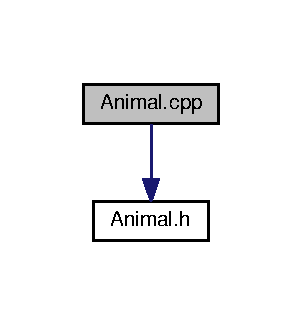
\includegraphics[width=145pt]{_animal_8cpp__incl}
\end{center}
\end{figure}

\hypertarget{_animal_8h}{}\section{Animal.\+h File Reference}
\label{_animal_8h}\index{Animal.\+h@{Animal.\+h}}
This graph shows which files directly or indirectly include this file\+:
\nopagebreak
\begin{figure}[H]
\begin{center}
\leavevmode
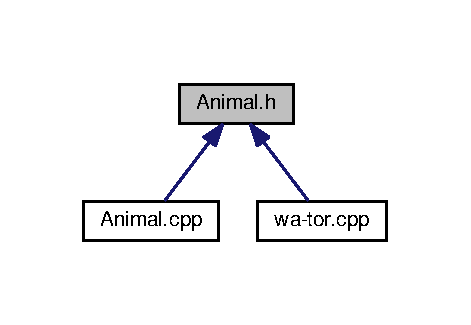
\includegraphics[width=226pt]{_animal_8h__dep__incl}
\end{center}
\end{figure}
\subsection*{Classes}
\begin{DoxyCompactItemize}
\item 
class \hyperlink{class_animal}{Animal}
\end{DoxyCompactItemize}

\hypertarget{_r_e_a_d_m_e_8md}{}\section{R\+E\+A\+D\+M\+E.\+md File Reference}
\label{_r_e_a_d_m_e_8md}\index{R\+E\+A\+D\+M\+E.\+md@{R\+E\+A\+D\+M\+E.\+md}}

\hypertarget{timer_8py}{}\section{timer.\+py File Reference}
\label{timer_8py}\index{timer.\+py@{timer.\+py}}
\subsection*{Namespaces}
\begin{DoxyCompactItemize}
\item 
 \hyperlink{namespacetimer}{timer}
\end{DoxyCompactItemize}
\subsection*{Variables}
\begin{DoxyCompactItemize}
\item 
int \hyperlink{namespacetimer_a5183291c63dada12162d2d2db5bc7c3c}{timer.\+loop\+\_\+times} = 100
\item 
\hyperlink{namespacetimer_ab45bd0f6c25534fef99fe5f87b0fb7e4}{timer.\+start\+\_\+time} = time.\+time()
\item 
\hyperlink{namespacetimer_aea0cd3f40ae910c8aae0c4dff8acb892}{timer.\+end\+\_\+time} = time.\+time()
\end{DoxyCompactItemize}

\hypertarget{wa-tor_8cpp}{}\section{wa-\/tor.cpp File Reference}
\label{wa-tor_8cpp}\index{wa-\/tor.\+cpp@{wa-\/tor.\+cpp}}
{\ttfamily \#include $<$iostream$>$}\\*
{\ttfamily \#include $<$fstream$>$}\\*
{\ttfamily \#include \char`\"{}Animal.\+h\char`\"{}}\\*
{\ttfamily \#include $<$stdio.\+h$>$}\\*
{\ttfamily \#include $<$stdlib.\+h$>$}\\*
{\ttfamily \#include $<$time.\+h$>$}\\*
{\ttfamily \#include $<$chrono$>$}\\*
{\ttfamily \#include $<$limits$>$}\\*
{\ttfamily \#include $<$unistd.\+h$>$}\\*
{\ttfamily \#include $<$iomanip$>$}\\*
Include dependency graph for wa-\/tor.cpp\+:
\nopagebreak
\begin{figure}[H]
\begin{center}
\leavevmode
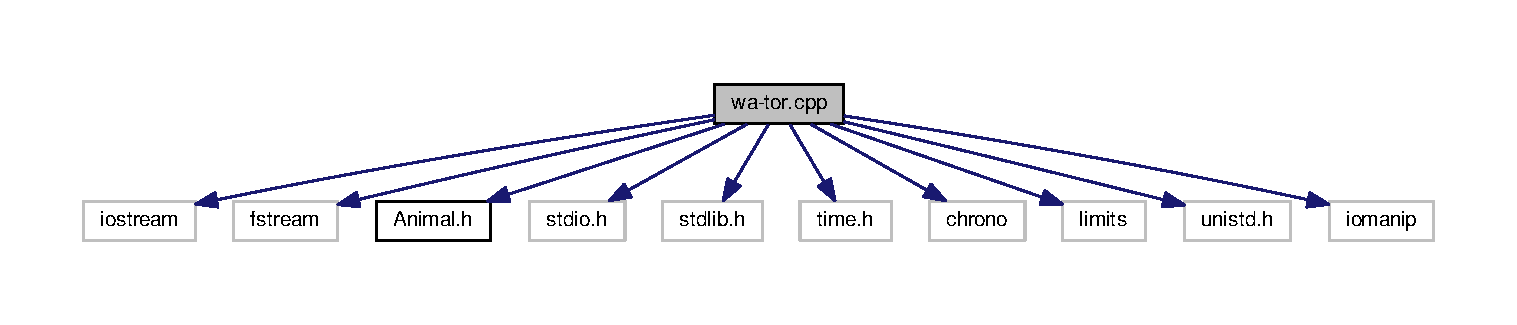
\includegraphics[width=350pt]{wa-tor_8cpp__incl}
\end{center}
\end{figure}
\subsection*{Functions}
\begin{DoxyCompactItemize}
\item 
void \hyperlink{wa-tor_8cpp_a87c9b3649865243c358781b9ba5a63ef}{write\+To\+File} (double \hyperlink{wa-tor_8cpp_a7cc6537125267d34b92ee58c7d5fa264}{finish\+Time})
\item 
int \hyperlink{wa-tor_8cpp_ac9c4c92d69ed70ac460b756440fc78ac}{find\+Partner} (int x, int y, int type, \hyperlink{class_animal}{Animal} temp\mbox{[}8\mbox{]})
\item 
void \hyperlink{wa-tor_8cpp_aa170cf839bf56d3c8a4b1e3ccf6885b9}{move\+Shark} (int i, int j)
\item 
void \hyperlink{wa-tor_8cpp_a89d4d5007ecb60011e978769f110d321}{move\+Fish} (int i, int j)
\item 
void \hyperlink{wa-tor_8cpp_a97e8c1c739a32ed95b9a7d50a53c52f7}{populate\+Map} ()
\item 
bool \hyperlink{wa-tor_8cpp_a9b90639a814dc879557d7ca2b4a8f188}{display\+Map} ()
\item 
void \hyperlink{wa-tor_8cpp_a9608986b5ab97722f2ebb5dccf5c83d2}{check\+Ocean} ()
\item 
int \hyperlink{wa-tor_8cpp_a662b974739cd0c3ab43007ea6530f4a8}{return\+Number} ()
\item 
int \hyperlink{wa-tor_8cpp_ae66f6b31b5ad750f1fe042a706a4e3d4}{main} ()
\end{DoxyCompactItemize}
\subsection*{Variables}
\begin{DoxyCompactItemize}
\item 
int const \hyperlink{wa-tor_8cpp_a586c34fe492dfaa733327c99e8cef1a7}{rows} = 35
\item 
int const \hyperlink{wa-tor_8cpp_a257ffd4af4f5b4a1792800a1da461fff}{columns} = 60
\item 
char \hyperlink{wa-tor_8cpp_a00bd8baeb581f6c8c6184c92b0514093}{map} \mbox{[}\hyperlink{wa-tor_8cpp_a586c34fe492dfaa733327c99e8cef1a7}{rows}\mbox{]}\mbox{[}\hyperlink{wa-tor_8cpp_a257ffd4af4f5b4a1792800a1da461fff}{columns}\mbox{]}
\item 
\hyperlink{class_animal}{Animal} \hyperlink{wa-tor_8cpp_ab8d425e802a7efbde7aee8ec63cf4109}{ocean} \mbox{[}\hyperlink{wa-tor_8cpp_a586c34fe492dfaa733327c99e8cef1a7}{rows}\mbox{]}\mbox{[}\hyperlink{wa-tor_8cpp_a257ffd4af4f5b4a1792800a1da461fff}{columns}\mbox{]}
\item 
int \hyperlink{wa-tor_8cpp_ae43dd048cc055db4f5afb2e51cda10d0}{fish\+Life} = 20
\item 
int \hyperlink{wa-tor_8cpp_a96baa8a35a57c2160fc29962b37e55b0}{shark\+Life} = 25
\item 
int \hyperlink{wa-tor_8cpp_a750943ec425a1b8104d0ed4a6f4073d3}{moves} = 0
\item 
int \hyperlink{wa-tor_8cpp_afe6bb1e77490b7b4d687dfebbffc0cba}{shark\+Breed} = 6
\item 
int \hyperlink{wa-tor_8cpp_a19573e234a78bbb14760f70a56297b97}{shark\+Starve} = 25
\item 
int \hyperlink{wa-tor_8cpp_a698d64c39d139b47bf8f1640d821b8b6}{fish\+Breed} = 2
\item 
int \hyperlink{wa-tor_8cpp_a8061b966958cc5112773ab457c12519f}{num\+Of\+Sharks} = 500
\item 
int \hyperlink{wa-tor_8cpp_a025064445afb61c29cfa42c27fe243ec}{num\+Of\+Fish} = 1000
\item 
double \hyperlink{wa-tor_8cpp_a7cc6537125267d34b92ee58c7d5fa264}{finish\+Time} = 0
\end{DoxyCompactItemize}


\subsection{Function Documentation}
\index{wa-\/tor.\+cpp@{wa-\/tor.\+cpp}!check\+Ocean@{check\+Ocean}}
\index{check\+Ocean@{check\+Ocean}!wa-\/tor.\+cpp@{wa-\/tor.\+cpp}}
\subsubsection[{\texorpdfstring{check\+Ocean()}{checkOcean()}}]{\setlength{\rightskip}{0pt plus 5cm}void check\+Ocean (
\begin{DoxyParamCaption}
{}
\end{DoxyParamCaption}
)}\hypertarget{wa-tor_8cpp_a9608986b5ab97722f2ebb5dccf5c83d2}{}\label{wa-tor_8cpp_a9608986b5ab97722f2ebb5dccf5c83d2}
Brief\+: Calls the turns for the animals \index{wa-\/tor.\+cpp@{wa-\/tor.\+cpp}!display\+Map@{display\+Map}}
\index{display\+Map@{display\+Map}!wa-\/tor.\+cpp@{wa-\/tor.\+cpp}}
\subsubsection[{\texorpdfstring{display\+Map()}{displayMap()}}]{\setlength{\rightskip}{0pt plus 5cm}bool display\+Map (
\begin{DoxyParamCaption}
{}
\end{DoxyParamCaption}
)}\hypertarget{wa-tor_8cpp_a9b90639a814dc879557d7ca2b4a8f188}{}\label{wa-tor_8cpp_a9b90639a814dc879557d7ca2b4a8f188}
Brief\+: Displays the current location of animals, and their count \index{wa-\/tor.\+cpp@{wa-\/tor.\+cpp}!find\+Partner@{find\+Partner}}
\index{find\+Partner@{find\+Partner}!wa-\/tor.\+cpp@{wa-\/tor.\+cpp}}
\subsubsection[{\texorpdfstring{find\+Partner(int x, int y, int type, Animal temp[8])}{findPartner(int x, int y, int type, Animal temp[8])}}]{\setlength{\rightskip}{0pt plus 5cm}int find\+Partner (
\begin{DoxyParamCaption}
\item[{int}]{x, }
\item[{int}]{y, }
\item[{int}]{type, }
\item[{{\bf Animal}}]{temp\mbox{[}8\mbox{]}}
\end{DoxyParamCaption}
)}\hypertarget{wa-tor_8cpp_ac9c4c92d69ed70ac460b756440fc78ac}{}\label{wa-tor_8cpp_ac9c4c92d69ed70ac460b756440fc78ac}
Brief\+: Searches for an animal type that is the same as itself \index{wa-\/tor.\+cpp@{wa-\/tor.\+cpp}!main@{main}}
\index{main@{main}!wa-\/tor.\+cpp@{wa-\/tor.\+cpp}}
\subsubsection[{\texorpdfstring{main()}{main()}}]{\setlength{\rightskip}{0pt plus 5cm}int main (
\begin{DoxyParamCaption}
{}
\end{DoxyParamCaption}
)}\hypertarget{wa-tor_8cpp_ae66f6b31b5ad750f1fe042a706a4e3d4}{}\label{wa-tor_8cpp_ae66f6b31b5ad750f1fe042a706a4e3d4}
std\+::cout $<$$<$ \char`\"{}\+Enter in number of sharks wanted\+: \char`\"{}; num\+Of\+Sharks = \hyperlink{wa-tor_8cpp_a662b974739cd0c3ab43007ea6530f4a8}{return\+Number()};

std\+::cout $<$$<$ \char`\"{}\+Enter in breed time of sharks wanted\+: \char`\"{}; shark\+Breed = \hyperlink{wa-tor_8cpp_a662b974739cd0c3ab43007ea6530f4a8}{return\+Number()};

std\+::cout $<$$<$ \char`\"{}\+Enter in starve time of sharks wanted\+: \char`\"{}; shark\+Starve = \hyperlink{wa-tor_8cpp_a662b974739cd0c3ab43007ea6530f4a8}{return\+Number()};

std\+::cout $<$$<$ \char`\"{}\+Enter in number of fishies wanted\+: \char`\"{}; num\+Of\+Fish = \hyperlink{wa-tor_8cpp_a662b974739cd0c3ab43007ea6530f4a8}{return\+Number()};

std\+::cout $<$$<$ \char`\"{}\+Enter in breed time of fish wanted\+: \char`\"{}; fish\+Breed = \hyperlink{wa-tor_8cpp_a662b974739cd0c3ab43007ea6530f4a8}{return\+Number()};

Puts animals into the map

execute while under 800 turns \index{wa-\/tor.\+cpp@{wa-\/tor.\+cpp}!move\+Fish@{move\+Fish}}
\index{move\+Fish@{move\+Fish}!wa-\/tor.\+cpp@{wa-\/tor.\+cpp}}
\subsubsection[{\texorpdfstring{move\+Fish(int i, int j)}{moveFish(int i, int j)}}]{\setlength{\rightskip}{0pt plus 5cm}void move\+Fish (
\begin{DoxyParamCaption}
\item[{int}]{i, }
\item[{int}]{j}
\end{DoxyParamCaption}
)}\hypertarget{wa-tor_8cpp_a89d4d5007ecb60011e978769f110d321}{}\label{wa-tor_8cpp_a89d4d5007ecb60011e978769f110d321}
Brief\+: Does the fish turn \index{wa-\/tor.\+cpp@{wa-\/tor.\+cpp}!move\+Shark@{move\+Shark}}
\index{move\+Shark@{move\+Shark}!wa-\/tor.\+cpp@{wa-\/tor.\+cpp}}
\subsubsection[{\texorpdfstring{move\+Shark(int i, int j)}{moveShark(int i, int j)}}]{\setlength{\rightskip}{0pt plus 5cm}void move\+Shark (
\begin{DoxyParamCaption}
\item[{int}]{i, }
\item[{int}]{j}
\end{DoxyParamCaption}
)}\hypertarget{wa-tor_8cpp_aa170cf839bf56d3c8a4b1e3ccf6885b9}{}\label{wa-tor_8cpp_aa170cf839bf56d3c8a4b1e3ccf6885b9}
Brief\+: Does the sharks turn \index{wa-\/tor.\+cpp@{wa-\/tor.\+cpp}!populate\+Map@{populate\+Map}}
\index{populate\+Map@{populate\+Map}!wa-\/tor.\+cpp@{wa-\/tor.\+cpp}}
\subsubsection[{\texorpdfstring{populate\+Map()}{populateMap()}}]{\setlength{\rightskip}{0pt plus 5cm}void populate\+Map (
\begin{DoxyParamCaption}
{}
\end{DoxyParamCaption}
)}\hypertarget{wa-tor_8cpp_a97e8c1c739a32ed95b9a7d50a53c52f7}{}\label{wa-tor_8cpp_a97e8c1c739a32ed95b9a7d50a53c52f7}
Brief\+: Creates map as empty \index{wa-\/tor.\+cpp@{wa-\/tor.\+cpp}!return\+Number@{return\+Number}}
\index{return\+Number@{return\+Number}!wa-\/tor.\+cpp@{wa-\/tor.\+cpp}}
\subsubsection[{\texorpdfstring{return\+Number()}{returnNumber()}}]{\setlength{\rightskip}{0pt plus 5cm}int return\+Number (
\begin{DoxyParamCaption}
{}
\end{DoxyParamCaption}
)}\hypertarget{wa-tor_8cpp_a662b974739cd0c3ab43007ea6530f4a8}{}\label{wa-tor_8cpp_a662b974739cd0c3ab43007ea6530f4a8}
Brief\+: Return the number input by the user \index{wa-\/tor.\+cpp@{wa-\/tor.\+cpp}!write\+To\+File@{write\+To\+File}}
\index{write\+To\+File@{write\+To\+File}!wa-\/tor.\+cpp@{wa-\/tor.\+cpp}}
\subsubsection[{\texorpdfstring{write\+To\+File(double finish\+Time)}{writeToFile(double finishTime)}}]{\setlength{\rightskip}{0pt plus 5cm}void write\+To\+File (
\begin{DoxyParamCaption}
\item[{double}]{finish\+Time}
\end{DoxyParamCaption}
)}\hypertarget{wa-tor_8cpp_a87c9b3649865243c358781b9ba5a63ef}{}\label{wa-tor_8cpp_a87c9b3649865243c358781b9ba5a63ef}
Brief \+: Writes the finish time to a file 

\subsection{Variable Documentation}
\index{wa-\/tor.\+cpp@{wa-\/tor.\+cpp}!columns@{columns}}
\index{columns@{columns}!wa-\/tor.\+cpp@{wa-\/tor.\+cpp}}
\subsubsection[{\texorpdfstring{columns}{columns}}]{\setlength{\rightskip}{0pt plus 5cm}int const columns = 60}\hypertarget{wa-tor_8cpp_a257ffd4af4f5b4a1792800a1da461fff}{}\label{wa-tor_8cpp_a257ffd4af4f5b4a1792800a1da461fff}
\index{wa-\/tor.\+cpp@{wa-\/tor.\+cpp}!finish\+Time@{finish\+Time}}
\index{finish\+Time@{finish\+Time}!wa-\/tor.\+cpp@{wa-\/tor.\+cpp}}
\subsubsection[{\texorpdfstring{finish\+Time}{finishTime}}]{\setlength{\rightskip}{0pt plus 5cm}double finish\+Time = 0}\hypertarget{wa-tor_8cpp_a7cc6537125267d34b92ee58c7d5fa264}{}\label{wa-tor_8cpp_a7cc6537125267d34b92ee58c7d5fa264}
\index{wa-\/tor.\+cpp@{wa-\/tor.\+cpp}!fish\+Breed@{fish\+Breed}}
\index{fish\+Breed@{fish\+Breed}!wa-\/tor.\+cpp@{wa-\/tor.\+cpp}}
\subsubsection[{\texorpdfstring{fish\+Breed}{fishBreed}}]{\setlength{\rightskip}{0pt plus 5cm}int fish\+Breed = 2}\hypertarget{wa-tor_8cpp_a698d64c39d139b47bf8f1640d821b8b6}{}\label{wa-tor_8cpp_a698d64c39d139b47bf8f1640d821b8b6}
\index{wa-\/tor.\+cpp@{wa-\/tor.\+cpp}!fish\+Life@{fish\+Life}}
\index{fish\+Life@{fish\+Life}!wa-\/tor.\+cpp@{wa-\/tor.\+cpp}}
\subsubsection[{\texorpdfstring{fish\+Life}{fishLife}}]{\setlength{\rightskip}{0pt plus 5cm}int fish\+Life = 20}\hypertarget{wa-tor_8cpp_ae43dd048cc055db4f5afb2e51cda10d0}{}\label{wa-tor_8cpp_ae43dd048cc055db4f5afb2e51cda10d0}
\index{wa-\/tor.\+cpp@{wa-\/tor.\+cpp}!map@{map}}
\index{map@{map}!wa-\/tor.\+cpp@{wa-\/tor.\+cpp}}
\subsubsection[{\texorpdfstring{map}{map}}]{\setlength{\rightskip}{0pt plus 5cm}char map\mbox{[}{\bf rows}\mbox{]}\mbox{[}{\bf columns}\mbox{]}}\hypertarget{wa-tor_8cpp_a00bd8baeb581f6c8c6184c92b0514093}{}\label{wa-tor_8cpp_a00bd8baeb581f6c8c6184c92b0514093}
\index{wa-\/tor.\+cpp@{wa-\/tor.\+cpp}!moves@{moves}}
\index{moves@{moves}!wa-\/tor.\+cpp@{wa-\/tor.\+cpp}}
\subsubsection[{\texorpdfstring{moves}{moves}}]{\setlength{\rightskip}{0pt plus 5cm}int moves = 0}\hypertarget{wa-tor_8cpp_a750943ec425a1b8104d0ed4a6f4073d3}{}\label{wa-tor_8cpp_a750943ec425a1b8104d0ed4a6f4073d3}
\index{wa-\/tor.\+cpp@{wa-\/tor.\+cpp}!num\+Of\+Fish@{num\+Of\+Fish}}
\index{num\+Of\+Fish@{num\+Of\+Fish}!wa-\/tor.\+cpp@{wa-\/tor.\+cpp}}
\subsubsection[{\texorpdfstring{num\+Of\+Fish}{numOfFish}}]{\setlength{\rightskip}{0pt plus 5cm}int num\+Of\+Fish = 1000}\hypertarget{wa-tor_8cpp_a025064445afb61c29cfa42c27fe243ec}{}\label{wa-tor_8cpp_a025064445afb61c29cfa42c27fe243ec}
\index{wa-\/tor.\+cpp@{wa-\/tor.\+cpp}!num\+Of\+Sharks@{num\+Of\+Sharks}}
\index{num\+Of\+Sharks@{num\+Of\+Sharks}!wa-\/tor.\+cpp@{wa-\/tor.\+cpp}}
\subsubsection[{\texorpdfstring{num\+Of\+Sharks}{numOfSharks}}]{\setlength{\rightskip}{0pt plus 5cm}int num\+Of\+Sharks = 500}\hypertarget{wa-tor_8cpp_a8061b966958cc5112773ab457c12519f}{}\label{wa-tor_8cpp_a8061b966958cc5112773ab457c12519f}
\index{wa-\/tor.\+cpp@{wa-\/tor.\+cpp}!ocean@{ocean}}
\index{ocean@{ocean}!wa-\/tor.\+cpp@{wa-\/tor.\+cpp}}
\subsubsection[{\texorpdfstring{ocean}{ocean}}]{\setlength{\rightskip}{0pt plus 5cm}{\bf Animal} ocean\mbox{[}{\bf rows}\mbox{]}\mbox{[}{\bf columns}\mbox{]}}\hypertarget{wa-tor_8cpp_ab8d425e802a7efbde7aee8ec63cf4109}{}\label{wa-tor_8cpp_ab8d425e802a7efbde7aee8ec63cf4109}
\index{wa-\/tor.\+cpp@{wa-\/tor.\+cpp}!rows@{rows}}
\index{rows@{rows}!wa-\/tor.\+cpp@{wa-\/tor.\+cpp}}
\subsubsection[{\texorpdfstring{rows}{rows}}]{\setlength{\rightskip}{0pt plus 5cm}int const rows = 35}\hypertarget{wa-tor_8cpp_a586c34fe492dfaa733327c99e8cef1a7}{}\label{wa-tor_8cpp_a586c34fe492dfaa733327c99e8cef1a7}
\index{wa-\/tor.\+cpp@{wa-\/tor.\+cpp}!shark\+Breed@{shark\+Breed}}
\index{shark\+Breed@{shark\+Breed}!wa-\/tor.\+cpp@{wa-\/tor.\+cpp}}
\subsubsection[{\texorpdfstring{shark\+Breed}{sharkBreed}}]{\setlength{\rightskip}{0pt plus 5cm}int shark\+Breed = 6}\hypertarget{wa-tor_8cpp_afe6bb1e77490b7b4d687dfebbffc0cba}{}\label{wa-tor_8cpp_afe6bb1e77490b7b4d687dfebbffc0cba}
\index{wa-\/tor.\+cpp@{wa-\/tor.\+cpp}!shark\+Life@{shark\+Life}}
\index{shark\+Life@{shark\+Life}!wa-\/tor.\+cpp@{wa-\/tor.\+cpp}}
\subsubsection[{\texorpdfstring{shark\+Life}{sharkLife}}]{\setlength{\rightskip}{0pt plus 5cm}int shark\+Life = 25}\hypertarget{wa-tor_8cpp_a96baa8a35a57c2160fc29962b37e55b0}{}\label{wa-tor_8cpp_a96baa8a35a57c2160fc29962b37e55b0}
\index{wa-\/tor.\+cpp@{wa-\/tor.\+cpp}!shark\+Starve@{shark\+Starve}}
\index{shark\+Starve@{shark\+Starve}!wa-\/tor.\+cpp@{wa-\/tor.\+cpp}}
\subsubsection[{\texorpdfstring{shark\+Starve}{sharkStarve}}]{\setlength{\rightskip}{0pt plus 5cm}int shark\+Starve = 25}\hypertarget{wa-tor_8cpp_a19573e234a78bbb14760f70a56297b97}{}\label{wa-tor_8cpp_a19573e234a78bbb14760f70a56297b97}

%--- End generated contents ---

% Index
\backmatter
\newpage
\phantomsection
\clearemptydoublepage
\addcontentsline{toc}{chapter}{Index}
\printindex

\end{document}
